\begin{figure}
\begin{subfigure}{0.52\linewidth}
\centering
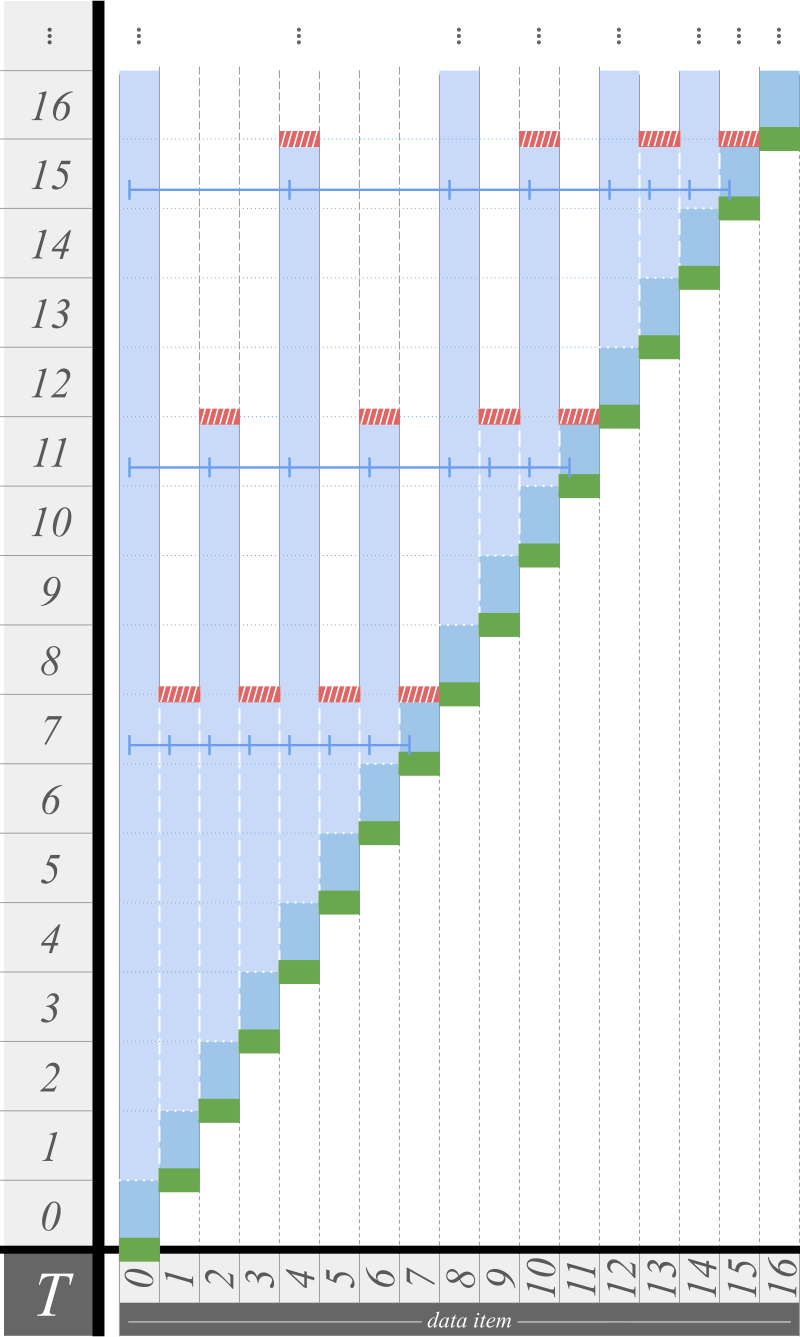
\includegraphics[height=2.7in,width=\linewidth]{img/surface-control-tall-zhao-tilted-doubling-naive-desat50}
\centering
\caption{\footnotesize naive doubling algorithm (Lst. \ref{alg:control-doubling-tilted})}
\label{fig:surface-control-tilted:naive-doubling}
\end{subfigure}
\begin{subfigure}{0.47\linewidth}
\centering
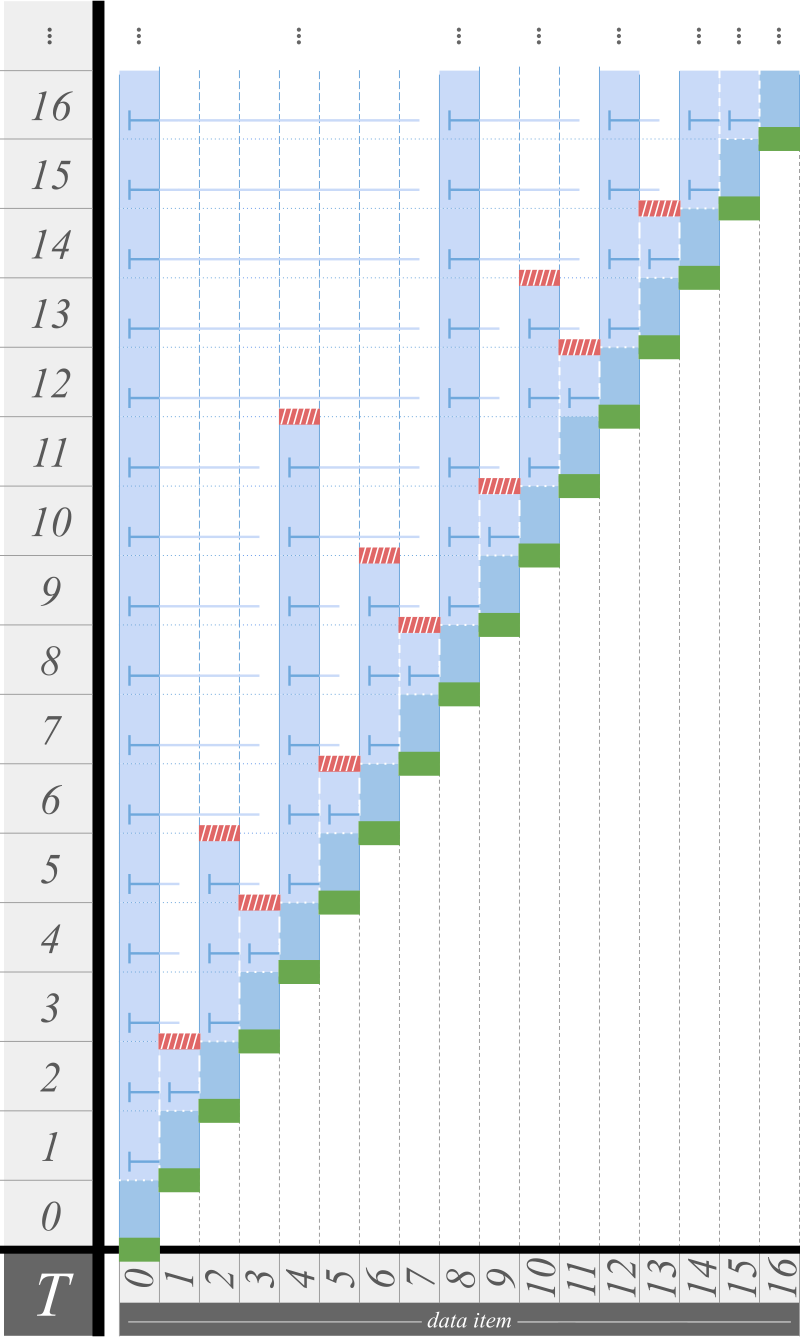
\includegraphics[height=2.7in,width=\linewidth,trim={2.5cm 0 0 0},clip]{img/surface-control-tall-zhao-desat50}
\centering
\caption{\footnotesize pyramidal bucket algorithm \citep{zhao2005generalized}}
\label{fig:surface-control-tilted:pyramidal}
\end{subfigure}

\begin{subfigure}{0.52\linewidth}
\centering
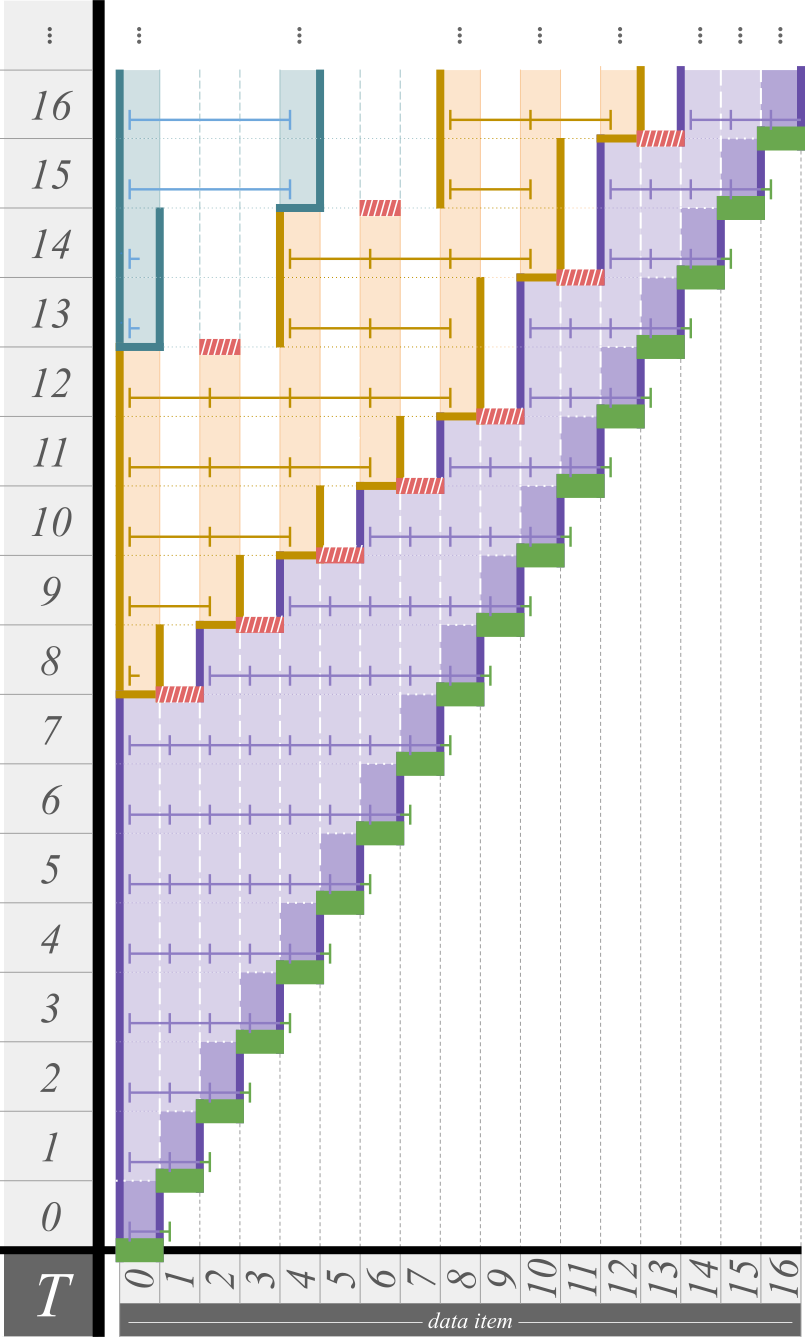
\includegraphics[height=2.7in,width=\linewidth,clip]{img/surface-control-tall-zhao-full-desat50}
\centering
\caption{\footnotesize saturating bucket algorithm (Lst. \ref{alg:zhao-tilted-full})}
\label{fig:surface-control-tilted:saturating-bucket}
\end{subfigure}%
\begin{minipage}{0.06\linewidth}
\centering ~
\end{minipage}%
\begin{minipage}[b]{0.42\linewidth}
\caption{%
\textbf{Comparator approaches for tilted curation.}
\footnotesize
Vertical segments correspond to duration between data item arrival (green bar) and deletion (red bar); time from bottom to top.
The naive doubling algorithm purges every other stored item when buffer space fills.
The pyramidal bucket algorithm organizes history into ``buckets'' of progressively doubling size (annotated), storing one item per bucket.
Each time step, the most recent pair of same-size buckets are merged.
The saturating bucket algorithm fills available space, divided among similarly-doubling ``buckets'' (color-coded by size).
The number of buckets within each size class (annotated) determines consolidation, which targets the most recent class more abundant than its successor.
}
\label{fig:surface-control-tilted}

\vspace{6ex}

\end{minipage}

% graphics from https://docs.google.com/presentation/d/1wUBwtvcawkSLw5TL-7d7jybp6TXB4Pi5s6FyXDcHB8M

\end{figure}
